
\subsection{Blockchain}
{A blockchain is a way of building a distributed ledger where the transactions that modify the ledger’s state are sequentially and immutably ordered by consensus. Therefore, Blockchain allows us to create a shared system to record what has happened. What has been recorded cannot be changed: it acts like a digital notary providing trust among parties. Note also that the information is shared because is built by different people, which is to say it is transparent and public. In addition, Blockchain technology, mainly the one based on smart contracts provides an extremely wide capability of programming our money.

In a blockchain, there are three main concepts: blocks, chains, and nodes. Block refers to data and state being stored in sequential groups of these blocks. To modify this state we have to perform a transaction of data, which needs to be added to a block to be finalized successfully. Furthermore, "chain" refers to each block referencing its parent. The data in each block cannot change without changing all subsequent blocks and would require the consensus of the whole network. Finally, the nodes refer to the computers which shape the network. They must agree upon each new block and the chain as a totality.

You can hear about a lot of benefits of using this technology such as data integrity, anonymity, reliability, etc. If we think about how it achieves all these properties we have to consider a combination of several ideas. Nodes are in charge of sharing the same state for everyone in the network. To achieve this, they negotiate through the consensus algorithm. }

\subsubsection{Source authentication, data integrity, and non-repudiation}
{We can start with how blockchain guarantees authentication and integrity. The public key cryptography plays a crucial role here. This algorithm is based on obtaining two keys, one public which is known by everybody and belongs to the user, and another private, which is known just by the owner. 

The private one is used to cipher a message, whereas the public one is used to decipher the message. This way, where someone decyphers the message with the public key it can verify that the message belongs to a certain owner since only he has the private key to do so, hence we get the \textbf{source authentication}.

Moreover, this data already signed cannot be modified, because I would need the private key to decipher and cypher again the message but the people just know the public key. So, just the private key owner can do this and we have achieved \textbf{data integrity} as well.

Note also that consequently, we are obtaining a very interesting property known as ``\textbf{non-repudiation}'', which merely refers to a situation where a statement's author cannot dispute its authorship.}

\subsubsection{One-way hash functions}
{Once we know how to protect data we have to think about the blockchain network. The objective of this network is to store data. This data can only be modified through transactions. Somehow, we are talking about a database. There is a basic requirement for a database which is a fast search capability. To achieve a great performance, it is applied one-way hash functions to the inputs, so the outputs are used as keys of the database. To decrease the capacity of that two different inputs generate a collision, i.e. generate the same hash, we are going to use really huge output space with 256 bits. Therefore, thanks to ``one-way hash functions'', given a hash output, it is computationally unfeasible to find the input.
More details about hashing are explained more deeply in appendix \ref{appendix:hashing}}.
\begin{figure}[H]
\centering
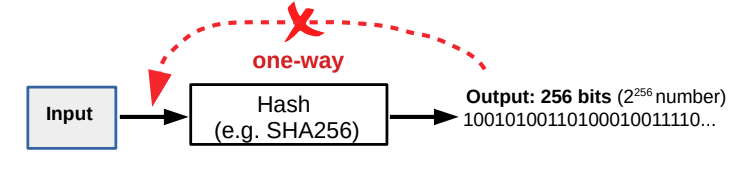
\includegraphics[width=12cm]{img/chapter_2/one-way-hash-functions.png}
\caption[One way functions]{\footnotesize{One way functions.}}
\label{fig:one-way-functions}
\end{figure}

\subsubsection{Transactions and consensus}
{Most of the ledgers that we usually use are centralized. All data is stored in a single computer and that makes it simple and it could be fast or convenient for an end user too. However, centralization has a drawback to consider: the power is centralized as well, and that is a risk if you cannot trust the owner. Banks are the typical example of this, but blockchain is attempting to offer a better solution. To do so, it relies on distributed systems, which are models in which components located on networked computers, \textbf{nodes}, communicate and coordinate their actions by passing messages. They have separated memories consolidating a shared state, where the ledger can be stored.

Now we are able to introduce how the ledger handles money. Users of the blockchain can create money movements, called \textbf{transactions}. All transactions are authenticated by their owners, even though we need \textbf{consensus}. The consensus is in charge of providing an order. This is fundamental in a ledger with the aim of avoiding negative balances. In a distributed system the consensus plays a main role since it has to ensure that the network avoids stuck states, stops if it is asynchronous, and progresses when the network recovers. Note that this means to force determinism, so external sources can just be injected as a transaction.

Another interesting property of money is to keep anonymity. Bank transfers are directly bound to the implied persons, whilst pocket money is not, so current digital transactions are not keeping this property. Blockchain pursues to resolve this too by creating an account ID that cannot be linked to a person. Users create a pair of public and private keys, sometimes the address is a derivation of the public key, and use that to sign the transactions on the network. Hence, everyone can have more than one account, and public keys have absolutely not any relation to the person's ID. 

Every blockchain has a different way of achieving consensus, in the case of Ethereum was accomplished initially thanks to \acrfull{pow} which was introduced by Bitcoin. Nevertheless, due to several reasons, Ethereum eventually migrated to \acrfull{pos} in 2022, which nowadays is a more common alternative and is increasing in popularity.

Both \acrlong{pow} and \acrlong{pos} are complex algorithms that are explained thoroughly in appendices \ref{appendix:proof-of-work} and \ref{appendix:proof-of-stake} respectively. It is a recommended reading in order to understand better the sense of consensus. 
}

\subsubsection{Cryptocurrencies}
{A cryptocurrency is an asset to exchange secured and trusted by a blockchain ledger. It represents a medium of exchange that is accepted as payment for goods and services. Blockchain allows users to make transactions over the network that would remain registered in the ledger without needing a third party to maintain them.

These cryptocurrencies are what the miners receive in compensation for the effort of mining new blocks and behaving honestly in the blockchain. This is the usual way the blockchain creates more tokens.

The first cryptocurrency was Bitcoin, created by Satoshi Nakamoto\cite{sathoshi}. Nowadays, thousands of blockchains and cryptocurrencies have appeared and evolved from Bitcoin.  }

\subsubsection{Wallets} \label{section:wallets}
{If a blockchain aims to process payments, every user will expect some software or hardware to interact with the network. Since there are many non-trivial concepts to take into account when interacting with the network, such a technology has to fit several requirements, some of which are the following: }
\begin{itemize}
    \item Show account balance, even in different currencies and blockchains.
    \item Manage multiple accounts.
    \item Manage user private keys: generate, backup, and so on.
    \item Send transactions and display transactions history.
\end{itemize}

{This item is what a \textbf{wallet} does.

Since wallets can manage a handful of accounts, and each one has its key pairs, they end up with a simple idea: Remember a single secret, which is the master, and derive all the key pairs from it. These types of wallets are called \textbf{Hierarchical Deterministic Wallets} \cite{hd-wallet}, or HD wallets. 

HD wallets ensure that all addresses needed are generated from a single seed instead of being randomly generated on demand, as you may see in figure \ref{fig:hierarchical-deterministic-wallet}. The seed is expressed in the form of a twelve-word seed-word phrase called \textbf{mnemonic}. Different public keys of the same HD wallet cannot be correlated unless you know the seed.}

\begin{figure}[H]
\centering
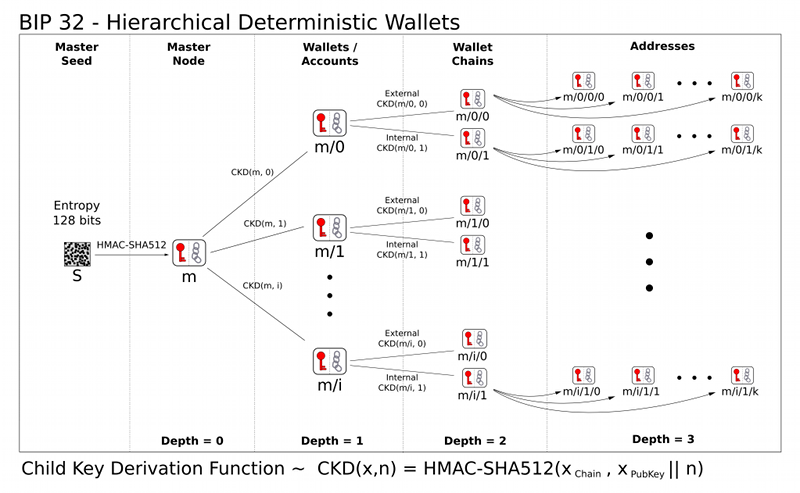
\includegraphics[width=14cm]{img/chapter_2/hierarchical-deterministic-wallet.png}
\caption[Hierarchical deterministic wallet]{\footnotesize{Hierarchical deterministic wallet.}}
\label{fig:hierarchical-deterministic-wallet}
\end{figure}

{One of the most popular software wallets is Metamask \cite{metamask}. Metamask is an HD wallet built as a browser extension that provides access to blockchain networks. When a user installs Metamask, it generates a random mnemonic and prompts the user to save it. Then, Metamask asks the user to introduce a password that will be used to encrypt the master secret and store it in the browser's local storage, which is known as \textit{vault}.


\begin{figure}[H]
\centering
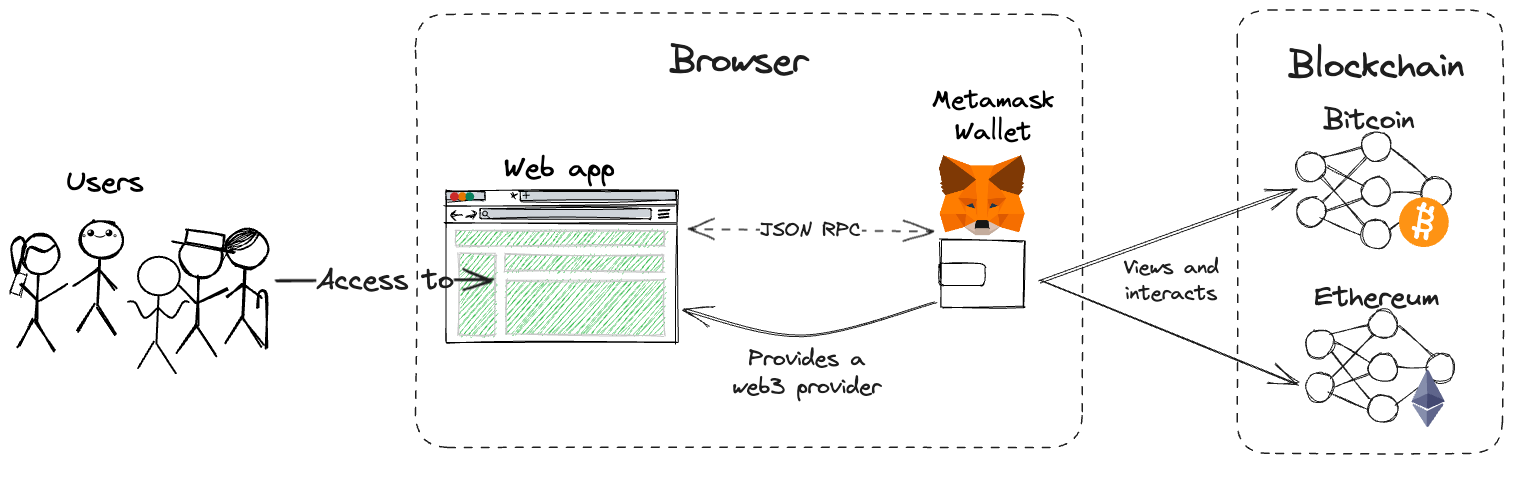
\includegraphics[width=14cm]{img/chapter_2/metamask-provider.png}
\caption[Metamask as web3 provider]{\footnotesize{Metamask as web3 provider.}}
\label{fig:metamask-mnemonic}
\end{figure}

As is illustrated in figure \ref{fig:metamask-mnemonic}, Metamask is designed to be a browser wallet. Wallets act as \textbf{web3 provider} to connect the different blockchains. The analogy is to think about this web3 provider as a telecom company offering you access to the cell network. Without such a provider, web applications would not be able to access the blockchains. This communication is carried out through the JSON-RPC protocol.}
